\documentclass{article}
\usepackage[paper=a4paper,margin=1in]{geometry}

\usepackage{listings}
\usepackage{graphicx}

\usepackage{comment}

%opening
\title{SProc Instruction Set Architecture}
\author{Ian O'Rourke}
\date{\today}

\begin{document}

\maketitle

\section{Overview}


SProc is a general-purpose Reduced Instruction Count (RISC) Instruction Set Architecture (ISA). Each program instruction is designed to take up exactly one word of memory. In this case, each word is 16-bits.

\subsection{Registers}

There are 16 total registers present on the SProc. These are defined generally as follows in Table \ref{table:register-setup}. Note that, as SProc is a 16-bit architecture, this means that each register is 16 bits wide.

\begin{table}[h!]
	\centering
	\begin{tabular}{c|c}
		\hline
		Register & Usage \\
		\hline
		R0 & Program Counter \\
		R1 & Global Stack Pointer \\
		R2 & Return Value \\
		R3-R15 & General Purpose Register \\
		\hline
	\end{tabular}
	\caption{Outside of the program counter and global stack pointer, the registers within the SProc are all general-purpose.}
	\label{table:register-setup}
\end{table}

\subsection{Overall Instruction Syntax}

Since the architecture of the SProc is 16-bit, this means that each word that may be addressed is 16-bits. The general instruction format is listed  in Table \ref{table:instruction-formatting}.

\begin{table}[h!]
	\centering
	\begin{tabular}{l|cccc}
		\hline
		Location & 0xF000 & 0x0F00 & 0x00F0 & 0x000F \\
		\hline
		Usage & opcode & arg0 & arg1 & arg2 \\
		\hline
	\end{tabular}
	\caption{The SProc instruction format typically has one opcode and three possible arguments associated with a particular opcode}
	\label{table:instruction-formatting}
\end{table}

This is contrasted with the typical assembly language formatting, which is provided as

\begin{center}
	\texttt{instruction <arg2>, <arg1>, <arg0>}
\end{center}

where the number of arguments depends on the required number of arguments for the instruction.

\subsection{Resetting}

On a hard-reset, all registers will be reset to 0 and memory values will be reset to their default values. The data parameter in memory at the hard-reset vector, stored at memory location 0, will be used as the reset vector.

On soft-reset, as called by the reset the program counter will be assigned the value contained in the soft-reset vector, which is stored at memory location 1. All of the other registers are reset to their default value of 0. Processor memory will be left unchanged and processor execution is then started.

On any reset, interrupts will be allowed by default.

\subsection{The Stack}

The stack pointer provides an offset from the stack pointer starting location. By default, this is at memory location 0x400. The stack pointer may grow up to a size of 0xC00, or 3072, items. If the stack pointer is ever popped such that its value would underflow 0 or would reach greater than the maximum allowed size, the processor will error and halt.

\subsection{Interrupts}

%TODO - Interrupt Items

\pagebreak

\section{Instructions and Assembly Code}

All available instructions are listed in Table \ref{table:instruction-table}. Note that any invalid instruction that is not provided in the table below results in an immediate halt of the processor.

\begin{table}[h!]
	\centering
	\begin{footnotesize}
		\begin{tabular}{cccc|c|l}
			\hline
			\multicolumn{4}{c|}{Instruction Word} & Assembly & Description \\
			opcode & arg0 & arg1 & arg2 & & \\
			\hline
			0 & 0 & 0 & 0 & \texttt{noop} & No Operation \\
			0 & 0 & 0 & 1 & \texttt{inton} & Turn Interrupts On \\
			0 & 0 & 0 & 2 & \texttt{intoff} & Turn Interrupts Off \\
			0 & 0 & 0 & 3 & \texttt{reset} & \texttt{PC = Reset Vector}, \texttt{R[0-15] = 0} \\
			0 & 0 & 0 & 4 & \texttt{pop} & \texttt{--SP} \\
			0 & 0 & 0 & 5 & \texttt{ret} & $\forall_{i \in [15 \rightarrow 0]}$ \texttt{R[i] = mem[--SP]}, \texttt{++PC} \\
			0 & 0 & 1 & R[a] & \texttt{jmp [a]} & \texttt{PC = R[a]} \\
			0 & 0 & 2 & R[a] & \texttt{jmpr [a]} & \texttt{PC += R[a]} \\
			0 & 0 & 3 & R[a] & \texttt{push [a]} & \texttt{mem[SP++] = R[a]} \\
			0 & 0 & 4 & R[a] & \texttt{popr [a]} & \texttt{R[a] = mem[--SP]} \\
			0 & 0 & 5 & R[a] & \texttt{call [a]} & $\forall_{i \in [0 \rightarrow 15]}$
			 \texttt{mem[SP++] = R[i]}, \texttt{PC = R[a]} \\
 			0 & 0 & 6 & R[a] & \texttt{int <imm>} & Trigger the Software Interrupt within vector <imm> \\
			0 & 1 & 0xI0 & 0x0I & \texttt{jmpri <imm>} & \texttt{PC += Im} \\
			0 & 2 & R[src] & R[dst] & \texttt{ld [dst], [src]} & \texttt{R[dst] = mem[R[src]]} \\
			0 & 3 & R[src] & R[dst] & \texttt{sav [dst], [src]} & \texttt{mem[R[dst]] = R[src]} \\
			0 & 4 & R[src] & R[dst] & \texttt{ldr [dst], [src]} & \texttt{R[dst] = mem[PC + R[src]]} \\
			0 & 5 & R[src] & R[dst] & \texttt{savr [dst], [src]} & \texttt{mem[PC + R[dst]] = R[src]} \\
			0 & 6 & R[cmp] & R[a] & \texttt{jz [a], [cmp]} & \texttt{PC = R[a] IF R[cmp] == 0} \\
			0 & 7 & R[cmp] & R[a] & \texttt{jzr [a], [cmp]} & \texttt{PC += R[a] IF R[cmp] == 0} \\
			0 & 8 & R[cmp] & R[a] & \texttt{jgz [a], [cmp]} & \texttt{PC = R[a] IF R[cmp] > 0} \\
			0 & 9 & R[cmp] & R[a] & \texttt{jgzr [a], [cmp]} & \texttt{PC += R[a] IF R[cmp] > 0} \\
			1 & 0xI0 & 0x0I & R[dst] & \texttt{ldi [dst], <imm>} & \texttt{R[dst] = Im} \\
			2 & 0xI0 & 0x0I & R[dst] & \texttt{ldui [dst], <imm-unsigned>} & \texttt{R[dst] = Im} \\
			3 & 0xI0 & 0x0I & R[dst] & \texttt{ldir [dst], <imm>} & \texttt{R[dst] = mem[PC + Im]} \\
			4 & R[b] & R[a] & R[dst] & \texttt{add [dst], [a], [b]} & \texttt{R[dst] = R[a] + R[b]} \\
			5 & R[b] & R[a] & R[dst] & \texttt{sub [dst], [a], [b]} & \texttt{R[dst] = R[a] - R[b]} \\
			6 & R[b] & R[a] & R[dst] & \texttt{mul [dst], [a], [b]} & \texttt{R[dst] = R[a] * R[b]} \\
			7 & R[b] & R[a] & R[dst] & \texttt{div [dst], [a], [b]} & \texttt{R[dst] = R[a] / R[b]} \\
			8 & R[b] & R[a] & R[dst] & \texttt{mod [dst], [a], [b]} & \texttt{R[dst] = R[a] \% R[b]} \\
			9 & R[b] & R[a] & R[dst] & \texttt{band [dst], [a], [b]} & \texttt{R[dst] = R[a] \& R[b]} \\
			10 & R[b] & R[a] & R[dst] & \texttt{bor [dst], [a], [b]} & \texttt{R[dst] = R[a] | R[b]} \\
			11 & R[b] & R[a] & R[dst] & \texttt{bxor [dst], [a], [b]} & \texttt{R[dst] = R[a] $\wedge$ R[b]} \\
			12 & R[b] & R[a] & R[dst] & \texttt{bsftl [dst], [a], [b]} & \texttt{R[dst] = R[a] << R[b]} \\
			13 & R[b] & R[a] & R[dst] & \texttt{bsftr [dst], [a], [b]} & \texttt{R[dst] = R[a] >> R[b]} \\
			\hline
		\end{tabular}
	\end{footnotesize}
	\caption{Available instruction list for the SProc provides a variety of commands.}
	\label{table:instruction-table}
\end{table}

The assembler also has several commands available, detailed in Table \ref{table:assembler-commands}.

\begin{table}[h!]
	\centering
	\begin{tabular}{l|l}
		\hline
		Command & Description \\
		\hline
		\texttt{:[label]} & Defines a new label associated with the current memory location \\
		\texttt{.oper [offset]} & Changes the current assembly offset to the value provided \\
		\texttt{.load [num]} & Loads the data value as either an unsigned word (if in hex or positive)\\
		& or as a signed word (if negative) in the current memory location \\
		\texttt{.loadloc [label]} & Loads the data index associated with the provided label into \\
		& the current memory location \\
		\hline
	\end{tabular}
	\caption{Available assembler commands}
	\label{table:assembler-commands}
\end{table}

Reference names are available to link to the special register values, as listed in Table \ref{table:assembler-register-references}.

\begin{table}[h!]
	\centering
	\begin{tabular}{l|cl}
		\hline
		Reference Name & Register & Description \\
		\hline
		\texttt{\$pc} & 0 & Program Counter \\
		\texttt{\$sp} & 1 & Stack Pointer \\
		\texttt{\$ret} & 2 & Return Value \\
		\hline
	\end{tabular}
	\caption{Assembler provides shortcuts for commonly-referenced register indices}
	\label{table:assembler-register-references}
\end{table}

\pagebreak

\section{Examples}

The following list some simple example programs that can be run on the SProc.

\subsection{Counter}

The program listed in Listing \ref{listing:example-counter} provides a basic counter. A target value is placed in register four, and the value in register three is incremented from 0 to the target value in register four by adding one to the register each loop. Once the target value has been reached and register three is equal to register four, the program halts by entering an infinite loop.

\lstinputlisting[caption={Limited counter program}, label={listing:example-counter}]{../examples/counter.smc}

Another simple program is provided in Listing \ref{listing:example-infinite-counter}. This program makes use of some additional functionality, including the use of the register reference names, to test register reset functionality. It also modifies the program counter outside of the standard jump command.

\lstinputlisting[caption={Infinite counter program with register reference names}, label={listing:example-infinite-counter}]{../examples/infinite_counter.smc}

\pagebreak

\section{Tools}

Several tools can help in the development of SProc programs.

\subsection{VisualSProc}

One useful tool is VisualSProc, which is a program that combines together a basic assembler, CPU emulator, and memory inspector into a single program. The main window can be seen in Figure \ref{fig:visual-sproc-main-page}.

\begin{figure}[h!]
	\centering
	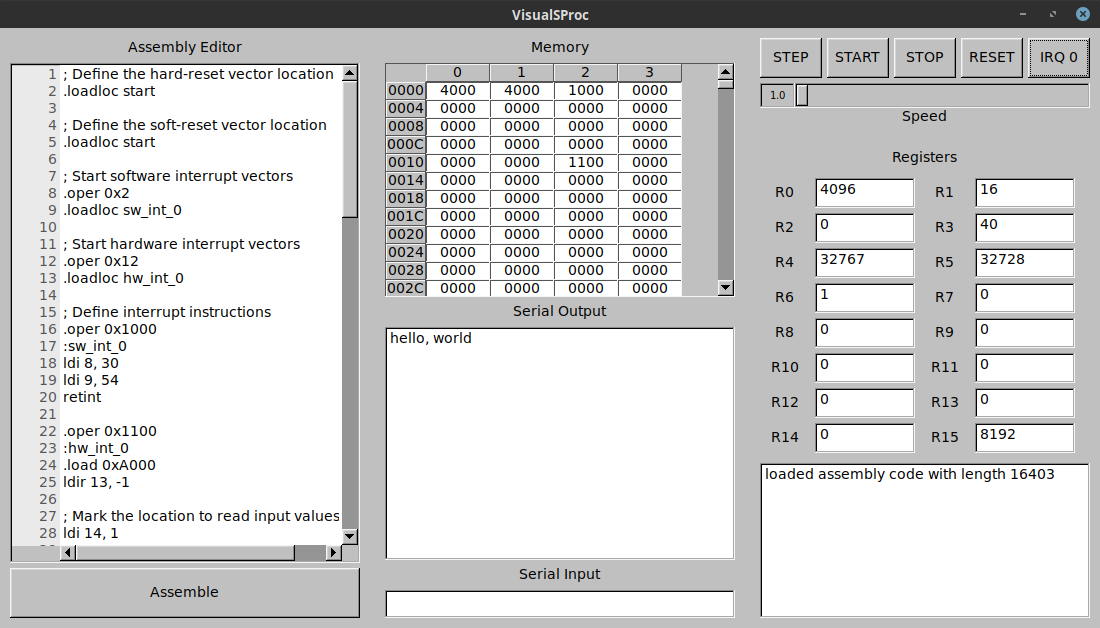
\includegraphics[width=5in]{images/visual-sproc.png}
	\caption{Main window of VisualSProc provides common tools for program writing}
	\label{fig:visual-sproc-main-page}
\end{figure}


\end{document}
